\documentclass[12pt]{article}
\usepackage[margin=0.5in]{geometry}



\usepackage{graphicx}
%\usepackage{amsmath}
%\usepackage{amsfonts}
%\usepackage{amssymb}
%\usepackage{amsthm}
%\usepackage{multicol}
%\usepackage{algorithms}
%\usepackage{showkeys}

%\newtheorem{Definition}{Definition}
%\newtheorem{Lemma}{Lemma}
%\newtheorem{Corollary}{Corollary}
%\newtheorem{Proposition}{Proposition}
%\newtheorem{Theorem}{Theorem}
%\newtheorem{Conjecture}{Conjecture}
%\newtheorem{Remark}{Remark}
%\newtheorem{question}{Question}
%\newtheorem{QaA}[question]{Q\&A}


\begin{document}

\title{Angry Ants: Progress Report}
%\date{\today}
\author{Jasmin Uribe and Yunhao Xu}
\maketitle
\section{Jan 29 2013}
\begin{itemize}
\item Updated project plan document, including locating (a subset of) relevant papers
\item Obtained data file from Yunhao, started writing code to process data
\item Started preliminary work on pilot experiments for the MC Basic algorithm
\item Began thinking about experiments that need to be run in order to implement shotgun algorithm
\end{itemize}

\section{Feb 5 2013}
\begin{itemize}
\item Continued writing code to process data
\item Discussed what information the trajectory graph needs to contain and how to obtain this from the data files
\item Discussed Alon's algorithm tried generalize to an arbitrary number of ants
\item Began formalizing shotgun sequencing algorithm, still brainstorming on a good way to initialize ants at different start times
\end{itemize}

\section{Feb 12 2013}
\begin{itemize}
\item Continued writing code to process data; code takes in trajectories in text files and finds clusters (ie. intersection points)
\item Currently working on processing these clusters into a graph 
\item Found python library for data analysis including min-cost
\item Discussed clustering parameters, ie. how close is considered an intersection point
\end{itemize}

\section{Feb 19 2013}
\begin{itemize}
 \item Continued working on processing path clusters into the trajectory graph
 \item Explored python library for data analysis
 \item Discussed how to test min-cost and greedy algorithms (current data set is essentialy only 1 `experiment', need more data sets)
\end{itemize}

\section{Feb 26 2013}
\begin{itemize}
 \item Continued working on creating trajectory graph
 \item Fleshed out shot-gun sequencing method (see below)
 \item Got access to local methods, will begin running and exploring the code
\end{itemize}
\subsection{Shot-gun sequencing method}
  Data must be gathered differently in order to implement this method. We already have `ground zero' trajectories for a second data set, we will use 
this to initialize each frame for the shot-gun method. We will randomly pick an ant to track (discrete uniform distribution). Using the ground truth
trajectory for this ant, we will randomly pick a time/location to initialize the game (discrete uniform distribution). The user will then track the ant from the specified time/place for 
a specified lenth of time. We will begin by having all users track for a fixed length of time (ie 30 sec), then we will have users track for a randomly
distributed length of time (Gaussian distribution). For each ant we will continue initializing at a new time/place until each time step has been tracked at least 3 times (note:
this parameter may change depending on data). Data for each ant will consist of a number, $n$, of mini-paths. Using these mini-paths and the time 
correspondence between them, we will `glue' the mini-paths together creating the final trajectory of the ant. We will determine the accuracy of the method by 
examining the Frechet distance and the least squares distance from the ground truth.
\subsection{Other Methods}
  Along with the shot-gun method we will also find the optimal trajectory for each ant using a simple greedy algorithm, a min-cost algorithm and the
Sergei/Alon linear programming algorithm. We will compare the results of all these algorithms, as well as the results from the local algorithms, to the 
ground truth. 
\subsection{Short term goals}
\begin{itemize}
 \item Explore local algorithms
 \item Email/meet with students working on Ants Game-provide them with specific details on how to initialize game for shot-gun method
 \item Finish creating trajectory graph for Data set 1 and run simple greedy and min-cost algorithms
\end{itemize}
\subsection{Longer goals}
\begin{itemize}
 \item Figure out exact details and write algorithm for how to process shot-gun data into full trajectories
 \item Generate random data set to test shot-gun method
 \item Run Sergei/Alon linear programming algorithm on data set 1, compare local/global for data set 1
 \item Once data set 2 collected, run all algorithms on data set 2 and compare
\end{itemize}

\section{March 19 2013}
\begin{itemize}
\item Read a multitude of papers relevant to research goals
\item Finished creating trajectory graph algorithm
\item Explored local methods
\item Explored implementing algorithms in Wiratma paper to use as comparison
\item Figured out what criteria defines a `good' median and how to measure 
\item Started measuring this criteria in implemented methods
\end{itemize}

\section{March 26 2013}
\begin{itemize}
\item Continued work on generating data similar to `real' data in order to test global algorithms
\item Set up meeting with Sergey to discuss data generation
\item Began searching for papers that include temporal component
\end{itemize}

\section{April 2 2013}
\begin{itemize}
\item Met with Sergey, Sankar, Lukas to discuss generting data-look for work on simulating paths
\item Looked at algorithms that generate 3D random walks--maybe use this to generate data
\item Met with Yunhao and discussed details about the project
\item Looked at current algorithms and discussed how portions can be used for our project
\item Set up goals for the week
\end{itemize}

\section{April 9 2013}
\begin{itemize}
\item	Work on the new ant data, create underline graph for greedy and ILP algorithm.
\item	Implement the greedy algorithm, prepare to compute the trajectories. (Have some bugs, not quite finished)
\item	Implement underline graph generator, including the ground graph and the user points.
\item	Compare underline graphs created by clustering algorithm with different threshold.
\end{itemize}

\section{April 16 2013}
\begin{itemize}
\item Finished implementing greedy algorithm
\item Created semi-random graph generator that forces an intersection at each time step
\item Created global graph using new data set- checking for possible bugs
\item Plan of attack- create random graphs and semi-random graphs, create user selections, use local algs, greedy and fuzzy k-means to extract median paths and compare to ground truth
\end{itemize}

\section{April 23 2013}
\begin{itemize}
\item We analyze our output from cluster \& greedy approach on the real data. According to the result, we believe this approach is at least as good as the automated and local approaches. (See Figure~\ref{fig1})
\item Generating plots, prepare for the final report.
\item We get around the "off screen" problem, by manually find out these frames and remove them away for particular ants. So if an ant went off screen between frame i to j, we make frame j+1 be the next frame of i-1 for that particular ant. We plan to get the data from the newest game with "off screen" option implemented, and run our test on that.
\end{itemize}
\begin{figure}[h]
\label{fig1}
 \begin{center}$
 \begin{array}{cc}
 \includegraphics[width=2.5in]{figure/range_50.png} &
 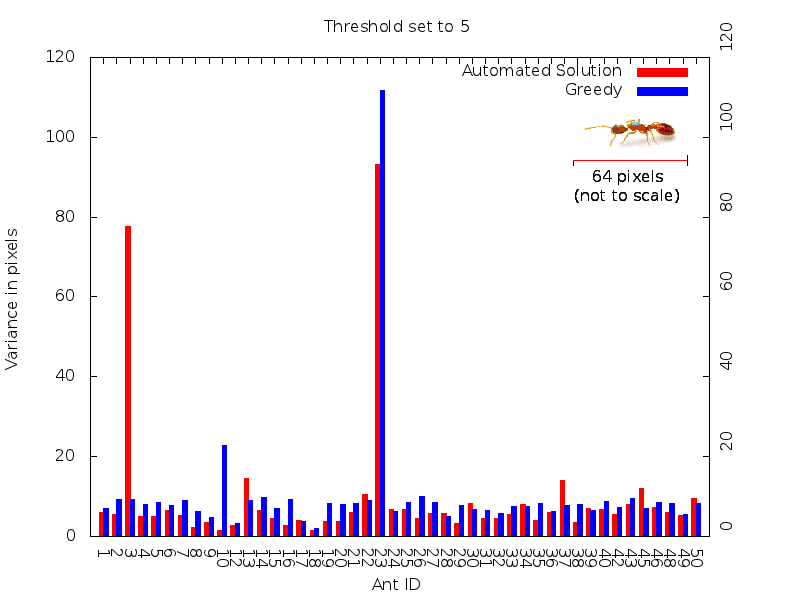
\includegraphics[width=2.5in]{figure/range_5.png}
 \end{array}$
 \end{center}
% \caption{}
 \end{figure}
\begin{figure}[h]
\label{fig2}
 \begin{center}
 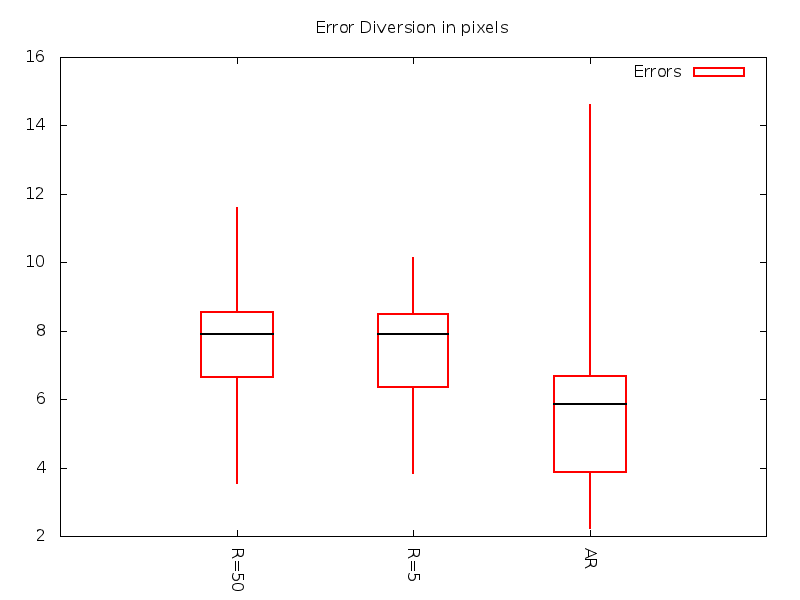
\includegraphics[width=2.5in]{figure/div.png}
 \end{center}
%  \caption{}
 \end{figure}

\end{document}